\section{Procedure}
\label{sec:procedure}

\subsection{Equipment}
The experimental setup is shown in Figure \ref{fig:MTS Machine}. The following equipment will be used to conduct the experiment:
\begin{figure}[h]
    \centering
    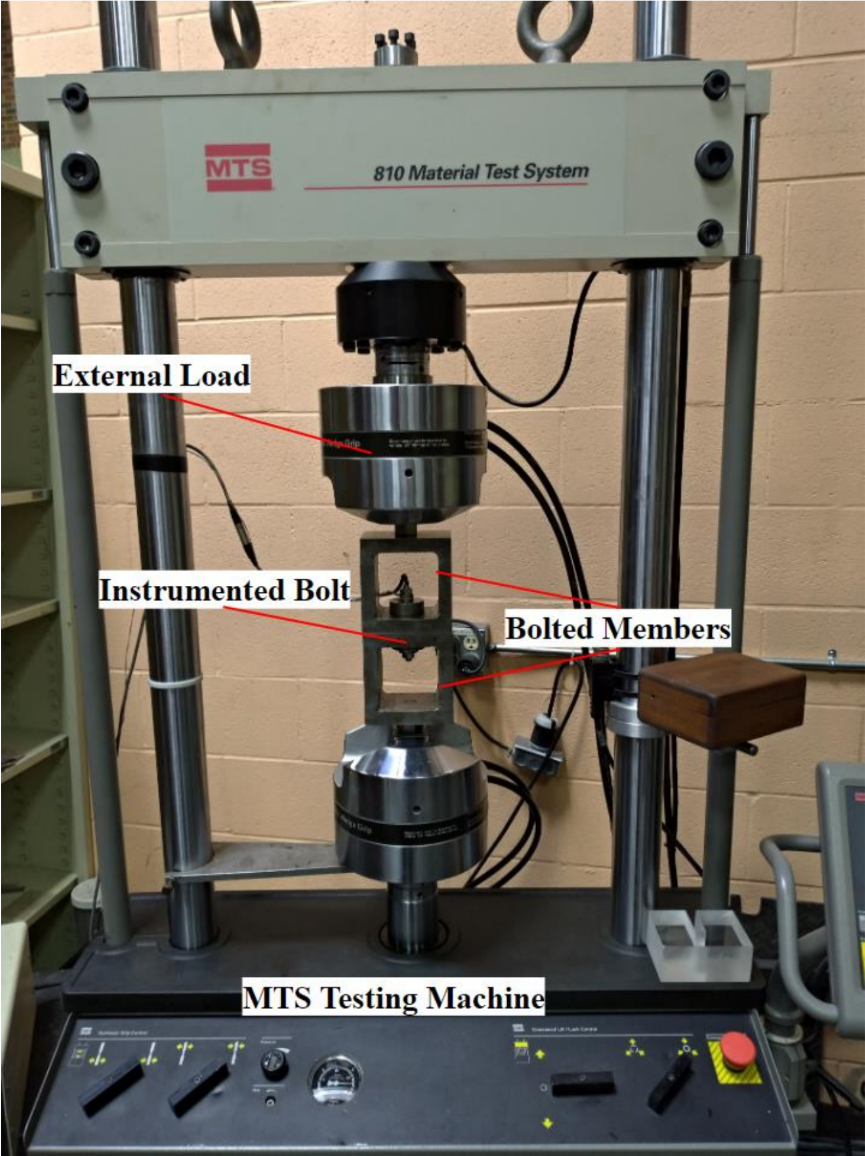
\includegraphics[width=0.3\textwidth]{Sections/Figures/MTS Machine.png}
    \caption{Experimental setup for bolted connection testing}
    \label{fig:MTS Machine}
\end{figure}
\begin{itemize}
    \item MTS testing machine, for applying controlled external loads to the bolted connection and measuring its response. The machine can also apply dynamic, or cyclic loads. 
    \item Instrumented bolt (Strainsert Type W), to output the bolt's strain as a voltage.
    \item Instrumented washer (Lebow Model 3711-375), to output the washer's strain as a voltage.
    \item Vishay strain gauge conditioner, to condition and amplify the signals from the strain gauges. 
    \item Torque wrench, for applying specific torque values to the bolt during preload and torque tests.
    \item Gasket of unknown material, the material will be analyzed during the experiment to determine its properties.
\end{itemize}


\subsection{Procedure}
\subsubsection{Zero Preload}
\begin{enumerate}
    \item Attach the bolted connection to the MTS machine with the nut attached "finger tight" (without a gasket).
    \item Load the bolt 8 times with a range of 0 - 7.5 kN.
    \item Record the external load and bridge imbalance at each load (0, 1, 2, 3, 4, 5, 6, 7, 7.5).
\end{enumerate}
\subsubsection{Repeatability Test}
\begin{enumerate}
    \item Attach the bolt to the MTS machine.
    \item Use the torque wrench to apply a preload of 50 in-lb.
    \item Record the voltage readings from the bolt and washer gauges.
    \item Loosen the bolt to remove any preload.
    \item Repeat steps 2-4 four more times.
\end{enumerate}
\subsubsection{Torque Test (Zero External Loading)}
\begin{enumerate}
    \item Attach the bolt to the MTS machine, without a gasket.
    \item Set the external load to 0 kN.
    \item Record the voltage readings from the bolt and washer gauges.
    \item Increase the torque by 25 in-lb.
    \item Record the voltage readings from the bolt and washer gauges.
    \item Repeat steps 4 and 5 four more times, obtaining readings from 0 to 125 in-lb of torque (0, 25, 50, 75, 100, 125).
\end{enumerate}
\subsubsection{Static Loading}
\begin{enumerate}
    \item Attach the bolt to the MTS machine (without a gasket).
    \item Tighten the bolt to 60 in-lb of torque.
    \item Set the external load on the MTS machine to 0 kN.
    \item Set the external load on the MTS machine to 7.5 kN.
    \item Record the readings from the bolt and washer.
    \item Repeat steps 3-5 two more times, totaling three readings (shakedown test).
    \item Leave the bolt assembled, and apply loads ranging from 0-7.5 kN (0, 1, 2, 3, 4, 5, 6, 7, 7.5). Record the output readings from the bolt and washer at each load.
    \item Set the load back to 0 kN.
    \item Disassemble and reassemble the joint with the gasket in place.
    \item Repeat steps 2-9 with a gasket.
\end{enumerate}
\subsubsection{Dynamic Loading}
\begin{enumerate}
    \item Attach the bolt to the MTS machine (without a gasket).
    \item Set the bolt to the "finger tight" torque setting.
    \item Apply an external load of 5 kN and an alternating load of 1.25 kN at 0.3 Hz.
    \item Record data for at least 10 cycles.
    \item Repeat steps 3-4 at different torque settings of 60, 75, and 125 in-lb.
    \item Disassemble and reassemble the joint with the gasket in place.
    \item Repeat steps 2-5 with a gasket.
\end{enumerate}
